\graphicspath{{img/ch2}}

\section{Lunar Pit Geological Characteristics}

\subsection{Morphological Characteristics}

Lunar pits exhibit distinct morphological features that provide critical insights into their geological origins and evolution. Typically characterized by funnel-shaped upper regions leading into near-vertical walls, these pits often terminate in flat or concave floors \cite{new-wagner, lunar-pits-numerical-modelling, lunar-pit-distribution}. The sharp transition between the sloping entrance and vertical walls suggests that these features form primarily due to sudden roof collapses above subsurface voids, rather than gradual erosion processes \cite{lunar-pits-numerical-modelling, new-wagner}.

\begin{figure}[h!]
    \centering
    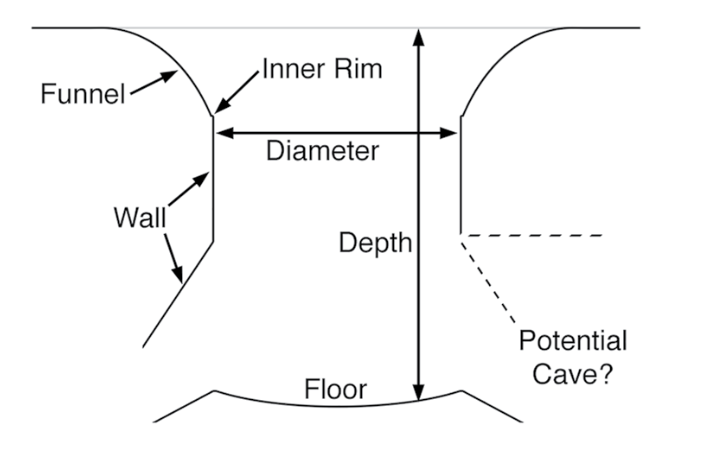
\includegraphics[width=0.5\linewidth]{lunar_pit_schema.png}
    \caption{A simplified schematic of a generic lunar pit cross-section showing key morphological features (adapted from \cite{new-wagner}).}
    \label{fig:lunar-pit-schema}
\end{figure}

High-resolution images from the Lunar Reconnaissance Orbiter (LRO) Narrow Angle Camera (NAC) have revealed significant details, such as layering within pit walls, which likely correspond to successive volcanic flow events. These layers serve as a geological record of ancient lunar volcanism \cite{new-wagner, lunar-pit-distribution}. Observations of overhangs within pits, such as those in Mare Tranquillitatis and Marius Hills, indicate access to subsurface voids consistent with collapsed lava tubes. These voids could extend tens of meters, offering compelling targets for future exploration \cite{lunar-pits-entrances-to-caves, Carrer2024}.

Boulder and regolith accumulations are commonly observed at the bases of lunar pits. Some pits exhibit concave floors, which contribute significantly to their depth and distinguish them from traditional impact craters, which are often characterized by raised rims and ejecta blankets \cite{lunar-pit-distribution, new-wagner}. 

\begin{figure}[H]
    \centering
    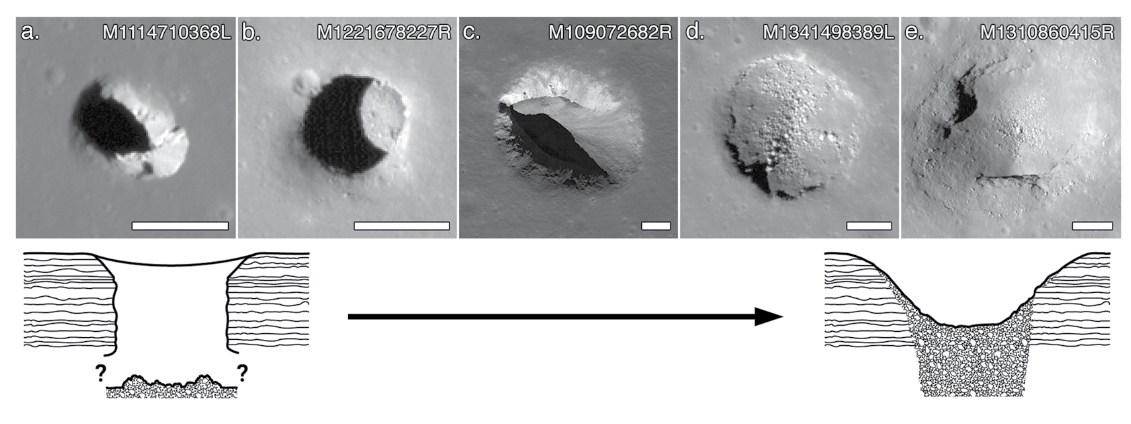
\includegraphics[width=0.85\linewidth]{closed_and_open_cavities.png}
    \caption{Progression of lunar pit degradation, illustrating gradual erosion and regolith deposition over time. Figure shows different lunar pits in various stages of erosion (adapted from \cite{new-wagner}).}
    \label{fig:lunar-pit-degradation}
\end{figure}

Over geological timescales, lunar pits degrade due to micrometeoroid impacts, thermal cycling, and seismic activity. These processes erode walls and rims, depositing debris at the base. Mare Tranquillitatis and Marius Hills pits demonstrate varying states of preservation, with sharper walls in younger pits and smoother, infilled floors in older examples. The degradation process appears largely independent of the surrounding terrain age, suggesting that pits evolve over hundreds of millions of years \cite{lunar-pit-distribution, radar-observations-lava-tubes}.

\subsection{Geographical Distribution and Formation Mechanisms}

Lunar pits are distributed across three primary geological settings: mare basalts, impact melt deposits, and highland terrain. Each setting reveals distinct formation mechanisms and geological implications \cite{lunar-pit-distribution, radar-observations-lava-tubes}.

\begin{figure}[H]
    \centering
    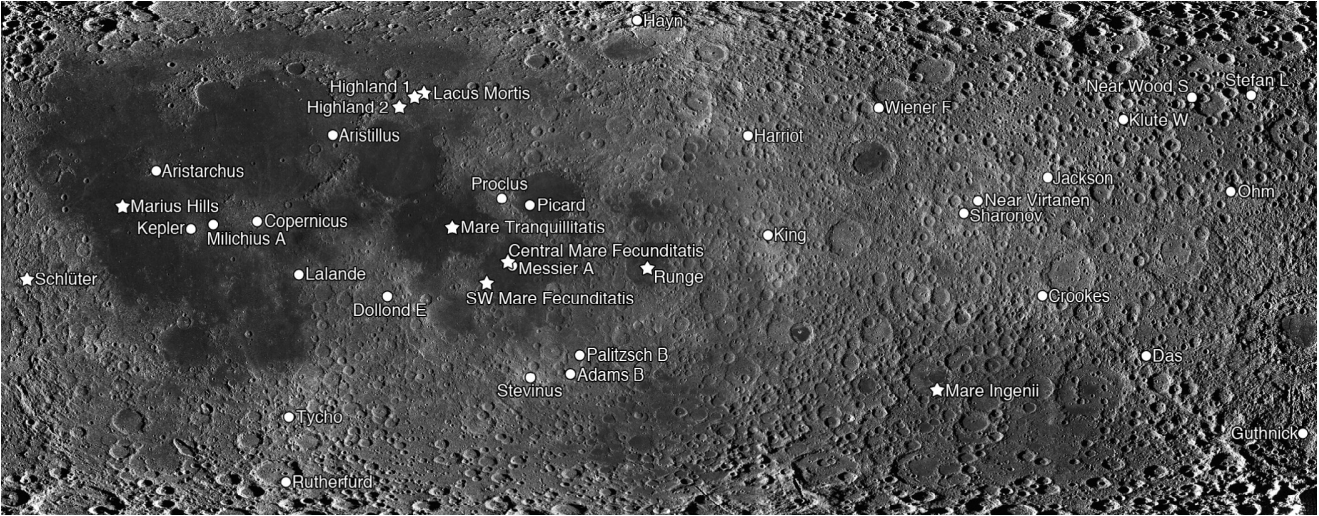
\includegraphics[width=0.76\linewidth]{map-lunar-pits-rough.png}
    \caption{Map of lunar pits: eight in mare basalts, two in highlands (stars), and 29 in impact melt deposits (dots). Figure adapted from \cite{lunar-pit-distribution}.}
    \label{fig:map-lunar-pits}
\end{figure}

\paragraph{Mare Basalts} 
Pits in mare regions, such as Marius Hills and Mare Tranquillitatis, are primarily associated with volcanic activity. These pits likely form due to the collapse of lava tube roofs, as overlying material becomes unstable and collapses into voids below \cite{lunar-pits-entrances-to-caves, radar-observations-lava-tubes}. Radar and imaging data from Mare Tranquillitatis reveal extensive subsurface voids consistent with intact lava tubes, which serve as potential habitats or scientific exploration targets \cite{Carrer2024, radar-observations-lava-tubes}.

\begin{figure}[H]
    \centering
    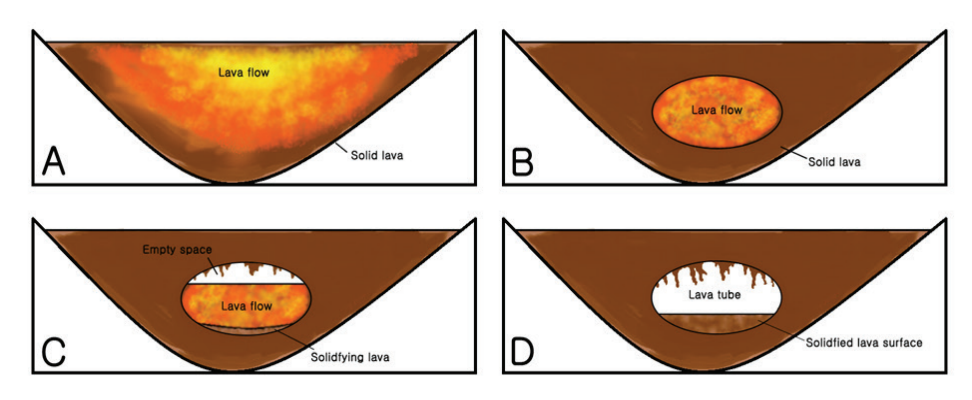
\includegraphics[width=0.7\linewidth]{lava_tube_formation_schema.png}
    \caption{Stages of lunar lava tube formation, illustrating crust solidification, lava drainage, and resulting voids (adapted from \cite{lunar-pits-entrances-to-caves}).}
    \label{fig:lava-tube-formation-schema}
\end{figure}

\paragraph{Impact Melt Deposits} 
Pits found within impact craters, such as Tycho and Copernicus, form due to high-energy impacts that fracture and compress the lunar crust, generating molten material. This molten material redistributes across the crater floor, and during solidification, thermal contraction creates cracks and fractures that eventually collapse into pits. These features are typically more circular in shape, lack overhangs, and have no association with lava flows \cite{clrn-impact-melt, lunar-pits-numerical-modelling}.

\begin{figure}[H]
    \centering
    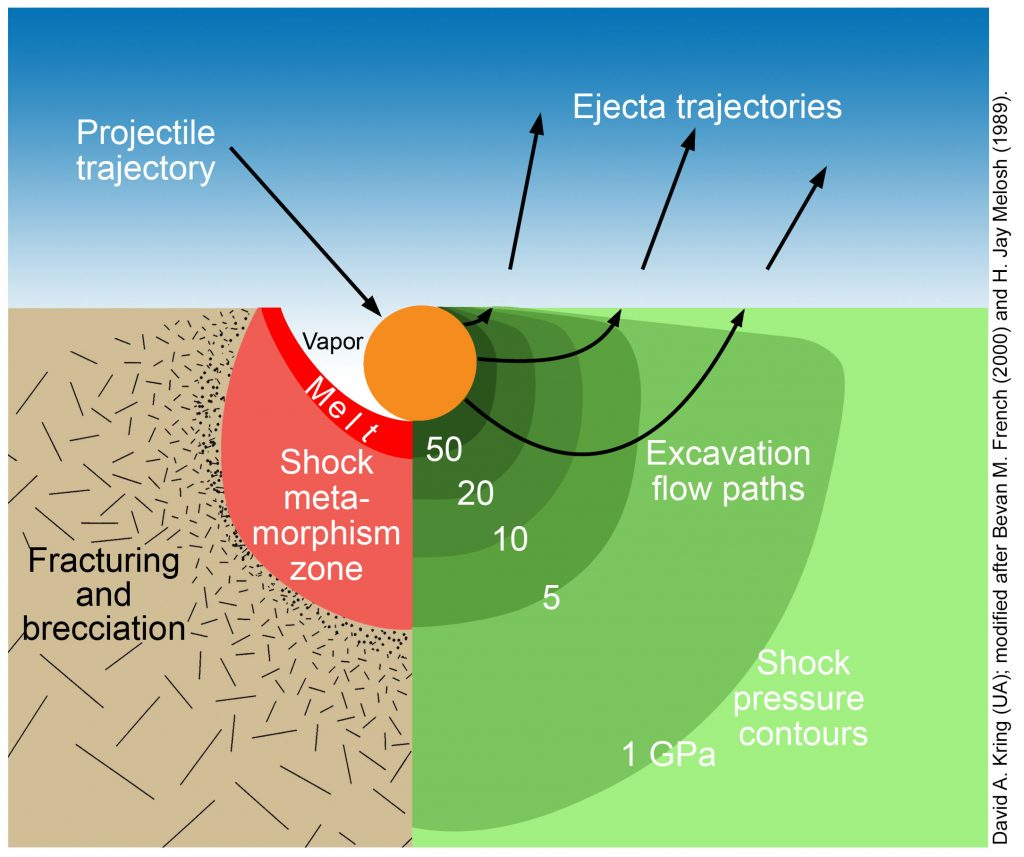
\includegraphics[width=0.42\linewidth]{Impact-Shock-Pressures-and-Their-Effects-1024x857.jpg}
    \caption{Impact dynamics illustrating pressure zones, molten material, and formation of cracks contributing to pit formation in impact melt deposits (adapted from \cite{clrn-impact-melt}).}
    \label{fig:impact-melt}
\end{figure}

\paragraph{Highland Terrain} 
Highland pits, such as those in Lacus Mortis, are thought to result from tectonic stress and extensional faulting. These pits typically form near graben systems or faulted regions, where crustal stress generates fractures. Over time, localized collapses along these fault zones create pits with sharp, near-vertical walls. Unlike mare pits, highland pits lack volcanic associations, emphasizing their tectonic origin \cite{new-wagner, lunar-pit-distribution}.

\begin{figure}[H]
    \centering
    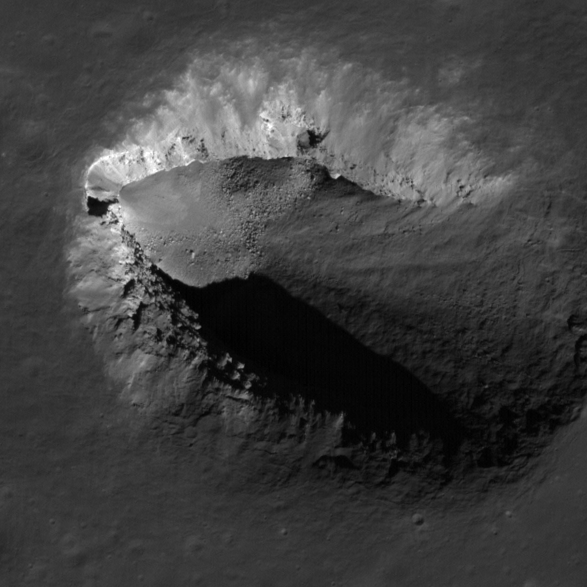
\includegraphics[width=0.33\linewidth]{lunar-pit-highland.png}
    \caption{Lunar Reconnaissance Orbiter Camera footage of Lacus Mortis Pit. Image adapted from: \url{https://www.lroc.asu.edu/atlases/pits}.}
    \label{fig:highland-lunar-pit}
\end{figure}

\paragraph{Impact-Induced Skylights}
These features form when small meteoroid impacts destabilize thin crusts overlying intact subsurface voids, such as lava tubes. Unlike traditional impact craters, skylights lack ejecta blankets and raised rims because the impact energy is localized, primarily collapsing the roof material. For instance, the Marius Hills pit formed from the collapse of a 26-meter-thick roof, creating a skylight approximately 40 meters wide \cite{clrn-impact-melt, lunar-pits-numerical-modelling}.

\begin{figure}[H]
    \centering
    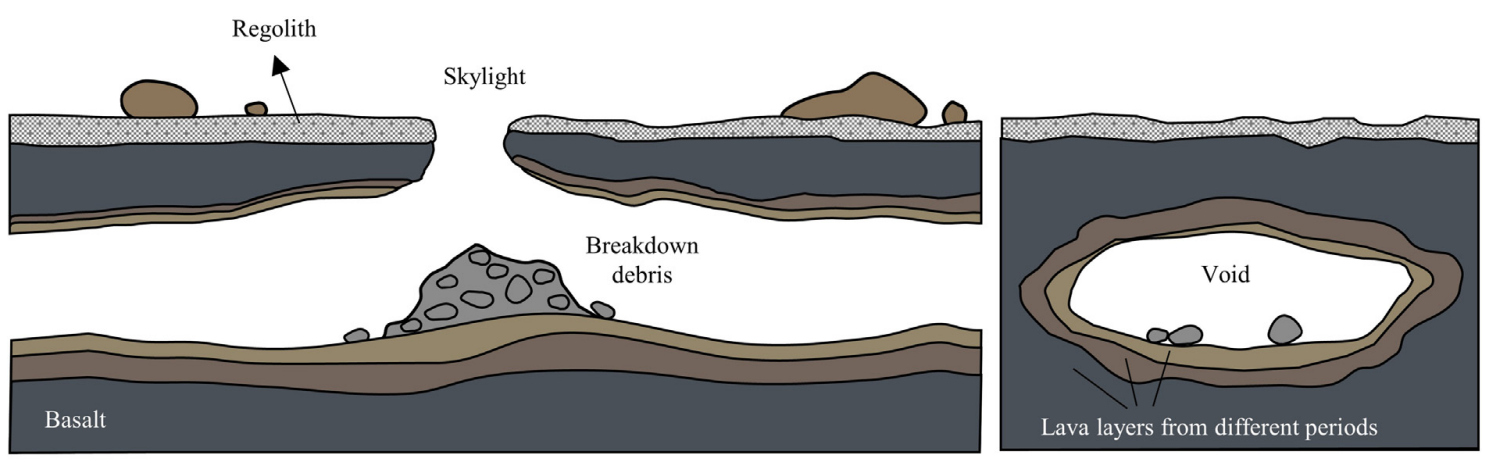
\includegraphics[width=0.99\linewidth]{lunar-pit-in-lava-tube.png}
    \caption{Cross section of a lunar tube with collapsed skylight (adapted from \cite{bases-feng}).}
    \label{fig:impact-induced-skylight}
\end{figure}
